%%%%%%%%%%%%%%%%%%%%%%%%%%%%%%%%%%%%%%%%%%%%%%%%%%%%%%%%%%%%%%%%%%%%%%%%%%%

\documentclass{standalone}

\usepackage{amsmath}
\usepackage{mathptmx}
\usepackage{pgfplots}
\usetikzlibrary{external}
\tikzexternalize{2x+1_x+3}
\pgfplotsset{compat=1.15}

%% IEEE uses Times Roman font, so we'll default to Times.
%% These three commands make up the entire times.sty package.
\renewcommand{\rmdefault}{ptm}
\renewcommand{\ttdefault}{pcr}
\normalfont\selectfont

\begin{document}

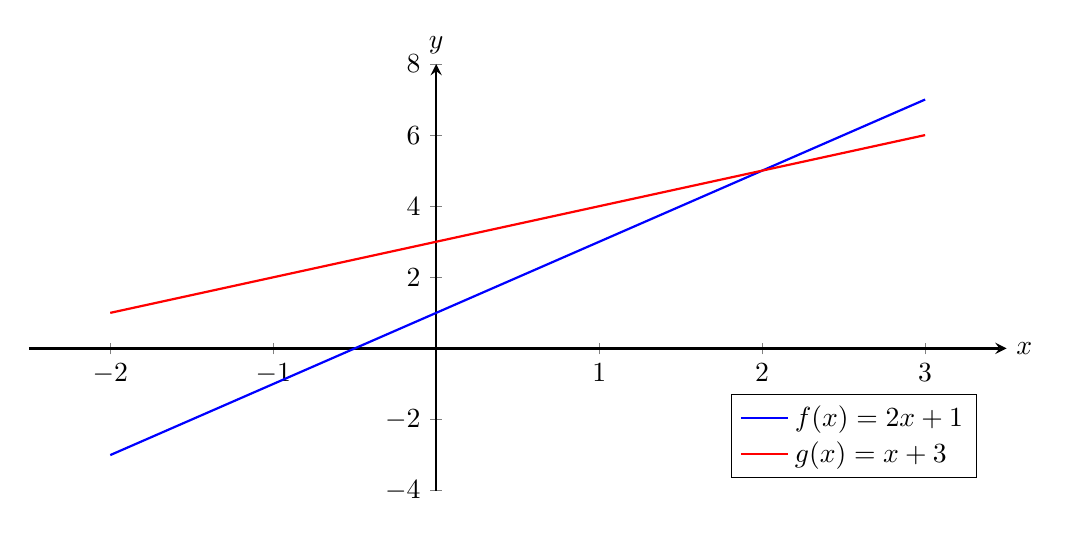
\begin{tikzpicture}
\tikzset{%%
  every mark/.append style={scale=1.0},%%
  scale=1.0%%
}
\pgfplotsset{%%
  every axis/.append style={font=\normalsize}%%
}
%%
\begin{axis}[%%
  axis line style=thick,%%
  axis lines=center,%%
  dotStyle/.style={only marks,mark size=2.5,black,mark color=black,mark=*},%%
  enlargelimits=true,%%
  height=7cm,%%
  legend cell align=left,%%
  legend pos={south east},%%
  plotStyle/.style={%%
    domain=-2:3,%%
    mark=none,%%
    smooth,%%
    thick%%
  },%%
  width=14cm,%%
  %%
  %% x-axis
  xlabel={\normalsize $x$},%%
  xlabel style={right},%%
  xtick={-2,-1,0,1,2,3},%%
  xticklabels={$-2$,$-1$,$0$,$1$,$2$,$3$},%%
  %%
  %% y-axis
  ylabel={\normalsize $y$},%%
  ylabel style=above%%
]
%%
%%
%% The function f(x) = 2x + 1.
\addplot+ [plotStyle]
{2*x + 1};
\addlegendentry{$f(x) = 2x + 1$}
%%
%% The function g(x) = x + 3.
\addplot+ [plotStyle]
{x + 3};
\addlegendentry{$g(x) = x + 3$}
\end{axis}
\end{tikzpicture}

\end{document}
